\chapter{Aktueller Forschungsstand}\label{forschungsstand}

Aktuell werden zwei verschiedene Ansätze verfolgt.
Entweder werden Photonen über Lichtwellenleiter an den Empfänger gesendet oder die Photonen werden durch die Luft gesendet.
Die zwei Methoden haben unterschiedliche Vor- und Nachteile, so ist die Übertragung durch einen Lichtwellen Leiter auf weniger 100km beschränkt und die Übertragung durch die Luft benötigt eine Strecke ohne feste, störende Objekte.

\begin{figure}[htbp] 
  \centering
     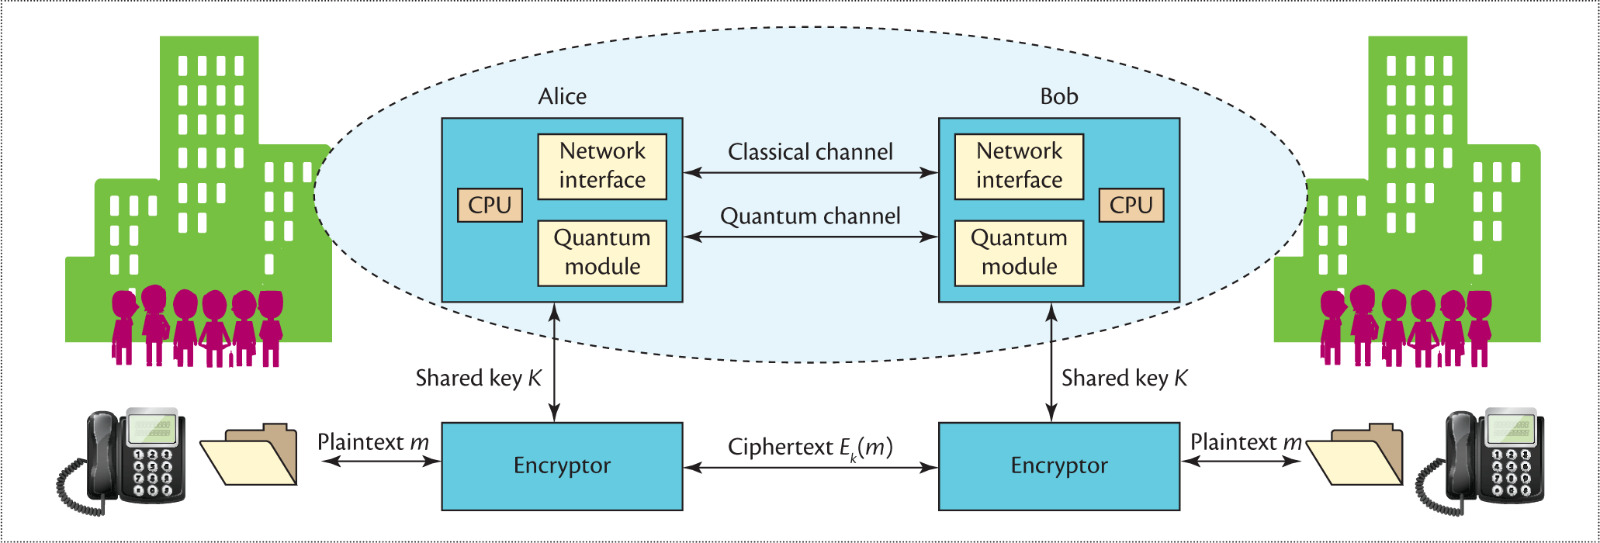
\includegraphics[width=0.9\textwidth]{img/qkd.jpg}
     \caption{Quantum Schlüsselaustausch (QKD) System. Die Architektur setzt sich zusammen aus einem Sender, Alice, und einem Empfänger, Bob, einem Optischen Quanten Kanal und einem Klassischen Kanal.}
  \label{fig:Bild1}
\end{figure}
\section{Air}
Das Kernverfahren der Quantenkryptographie liegt im Schlüsselaustausch
dieser dient, analog zu den konventionellen Verschlüsselungsverfahren, dem Austausch einer gemeinsamen Zufallszahl mit der ein zu übertragendes Signal verschlüsselt werden kann. Die Besonderheit liegt hier bei der sehr hohen Wahrscheinlichkeit den Schlüssel durch äußere Abhörversuche unbrauchbar zu machen, hiermit wird das direkte Abhören beim Schlüsselaustausch überflüssig. Im Englischen bezeichnet man besagte Verfahren als \ac{QKD}

Wie von \cite{Ren_2017} in Kooperation zwischen Wien und Shanghai bewiesen, lassen sich Photonen über Satelliten durch den quasi luftleeren Raum Störungsfreier und dadurch viel weiter übertragen. Im Falle der Studie von \cite{Ren_2017} wurde ein Schlüsselaustausch zwischen Wien und Shanghai über eine Strecke von 1120 Kilometer erreicht werden. Die aktuelle Übertragungsrate ist allerdings mit 0,12 Bit/s sehr gering. Hinzu kommt, dass die Übertragung, aufgrund der Störeffekte der Photonen des Sonnenlichts, nur Nachts möglich ist.

Forscher der Leibniz Universität Hannover haben zusammen mit Forschern der Universität Glasgow und des des japanischen NICT (National Institute of Information and Communications Technology) eine Möglichkeit der Übertragung verschränkter Photonen im Infrarotspektrum geschaffen \cite{prabhakar_two-photon_2020}. Diese Technologie nutzt das so genannte "atmosphärische Fenster" d.h. einen bestimmten Frequenzbereich bei dem sich die Atmosphäre lichtdurchlässiger verhält. Auch die Sonnenstrahlung ist im Infrarotbereich schwächer und stört die Übertragung weniger als im sichtbaren Bereich. Allerdings ist diese Methode noch weniger ausgereift und weißt bei der Detektion eine Rate von 2\% aller Übertragenen Photonen im Gegensatz zu 90\% bei der Methode von \cite{Ren_2017} auf.

\section{Lichtwellenleiter}

Die Standardmethode für verschlüsselte Kommunikation in Quantennetzwerken ist die \ac{QKD} über Fiberglas.
Hier wird die grundlegende Materie des Lichts, Photonen, übertragen um Informationen weiter zu geben.
Diese Übertragung kann nicht ohne Rauschen stattfinden, sodass ein Übertragung bis maximal 100 km möglich ist\cite{Shen2018}.

Des weiteren findet die Übertragung immer von einem Teilnehmer zu einem zweiten statt und ein Multicast, welcher eine Information von einem Sender an mehrere Empfänger schickt, ist in Quantennetzwerken mit \ac{QKD} nicht etabliert.
Stattdessen werden die Informationen individuell an jeden einzelnen Empfänger gesendet oder Daten werden von einem Verteiler an die verschiedenen Empfänger verteilt.
Dabei muss ein Schlüsselaustausch zwischen dem ersten Teilnehmer und dem Verteiler stattfinden und ein zweiter Schlüsselaustausch zwischen dem Verteiler und dem zweiten Teilnehmer.
Somit ist die Übertragung auf dem Verteiler unverschlüsselt und deshalb muss dem Verteiler vertraut werden\cite{Qiu2018}.

Dieses Jahr wurde ein Netzwerk zwischen acht Teilnehmern realisiert, welches mit multiplexern und demultiplexern arbeitet.
Das hat den Vorteil, dass keine aktives verteilen der einzelnen Daten geschehen muss\cite{Siddarth2020}.

Die Übertragung in einem Lichtwellenleiter kann dabei entweder im single-mode als auch im multi-mode stattfinden.
Beim single-mode wird ein einzelner Photonenstrahl vom Sender in den Lichtwellenleiter gegeben, was ein dünneres Kabel erlaubt.
Allerdings macht die mulit-mode Methode eine höhere Präzession möglich\cite{VanMeter2014}.
Beide Möglichkeiten werden aktuell schon in klassischen Netzwerken genutzt und sind weit verbreitet.

